\chapter{Leyes invariantes, cuatro-vectores y tensor de campo}

Comenzaremos con una ley que la naturaleza podría haber obedecido, pero no obedece. Su incumplimiento nos indicará cómo debe escribirse una ley física. Esta misma prueba nos lleva primero de las componentes de coordenadas a los vectores ordinarios, luego de estos a los cuatro-vectores y, por último, de los cuatro-vectores a los tensores. Al final, los campos eléctrico y magnético dejarán de ser objetos separados: juntos ocuparán las seis posiciones independientes de un único tensor antisimétrico.

Salvo que se indique lo contrario, usamos unidades en las que \(c=1\), ordenamos las componentes del espacio-tiempo como \((1,2,3,0)=(x,y,z,t)\) y usamos la signatura métrica \((-,-,-,+)\).

\section{Una posible ley con la simetría equivocada}

Fijemos permanentemente en el espacio un eje \(x\) y uno \(y\). Ahora establezcamos que dos partículas interactúan cuando sus coordenadas \(x\) coinciden. La interacción podría invertir su movimiento o hacer que partieran en nuevas direcciones; su dinámica detallada no importa. La condición que la desencadena es sencillamente \begin{equation}
  x_1-x_2=0,
\end{equation}, donde los subíndices identifican partículas, no componentes de coordenadas. Esta regla no encierra ninguna contradicción matemática. La pregunta es qué la hace físicamente poco plausible.

\begin{classroomqa}\audiencequestion{¿Viola la regla la homogeneidad del espacio?}\lecturerresponse{No. Trasladar el origen cambia ambas coordenadas en la misma cantidad y deja inalterado \(x_1-x_2\). La regla no especifica ningún lugar preferido. Su defecto es la isotropía: distingue una dirección preferida.}\end{classroomqa}

Giremos los ejes \(90^\circ\). Ahora llamamos \(y\) a la antigua dirección \(x\), de modo que los mismos sucesos físicos se describirían mediante la igualdad de las coordenadas \(y\). En un ángulo cualquiera, la condición incluiría una combinación lineal de \(x\) y \(y\). Por tanto, la forma de la ley depende de la orientación de la pizarra. Es invariante ante traslaciones, pero no ante rotaciones.

Solemos expresar las leyes físicas en su forma más sencilla usando coordenadas ortogonales. Se pueden usar coordenadas más generales, pero entonces la métrica y las fórmulas se vuelven menos sencillas. Dentro de la clase de marcos cartesianos ortogonales, ninguna orientación debe ser privilegiada.

La solución es inmediata. En dos dimensiones, exijamos que coincidan ambas coordenadas; en tres, las tres: \begin{equation}
  x_1=x_2,
  \qquad y_1=y_2,
  \qquad z_1=z_2.
\end{equation} Así, las partículas solo pueden interactuar cuando llegan al mismo punto, aunque se aproximen a él por líneas distintas.

\begin{classroomqa}\audiencequestion{¿También deben coincidir las coordenadas \(z\) y los tiempos?}\lecturerresponse{En el espacio tridimensional también deben coincidir las coordenadas \(z\). Por ahora dejamos de lado el tiempo; lo reincorporaremos en cuanto completemos el argumento espacial.}\end{classroomqa}

Sea \(\boldsymbol r_a\) la posición de la partícula \(a\). Las tres condiciones para las componentes se convierten en una ecuación vectorial: \begin{equation}
  \boldsymbol r_1-\boldsymbol r_2=\boldsymbol 0.
\end{equation} Una componente puede anularse en un marco rotado y no anularse en otro. El vector completo es distinto: si todas sus componentes son cero en un marco, también lo son en cualquier marco rotado. Del mismo modo, si dos vectores son iguales en un marco, siguen siéndolo después de transformar ambos.

\begin{figure}[H]\centering
\includegraphics[width=0.78\textwidth]{lecture_06_figure_01.png}\caption{Las tres igualdades de coordenadas que hacen que una colisión signifique coincidencia espacial, en vez de coincidencia a lo largo de un eje preferido.}\lectureframe{00:09:00}\end{figure}

Por eso son útiles las ecuaciones vectoriales. Sus componentes cambian, pero el objeto se transforma de manera coherente. Una ley expresada para el objeto completo puede conservar su forma cuando se rotan las coordenadas.

\section{Coincidencia en el espacio-tiempo}

Reemplacemos ahora el eje espacial vertical por el tiempo. Una regla newtoniana podría decir que dos cambios de movimiento solo ocurren en tiempos iguales. En la mecánica newtoniana, la simultaneidad es común a todos los observadores inerciales, así que tal regla es posible. En la relatividad especial, selecciona un marco preferido. Los sucesos simultáneos en un marco no tienen por qué serlo en otro.

Exigir solo la igualdad de las coordenadas espaciales no es mejor. Un desplazamiento espacio-temporal puede tener componentes espaciales nulas y una componente temporal distinta de cero: \begin{equation}
  \Delta X^\mu=(0,0,0,\Delta t),
\end{equation}, y una transformación de Lorentz mezcla \(\Delta t\) con una componente espacial. La afirmación local invariante es que los dos cambios de movimiento ocurren en el mismo suceso. Por tanto, una colisión simple exige \begin{equation}
  X_1^\mu=X_2^\mu,
  \qquad\text{or}\qquad
  X_1^\mu-X_2^\mu=0.
\end{equation} Las cuatro coordenadas coinciden: las partículas ocupan el mismo lugar en el mismo instante.

El ejemplo de la colisión da una regla general para formular la física. Podemos poner todo en un lado e igualar a cero un cuatro-vector completo, o igualar un cuatro-vector completo con otro. Igualar partes inconexas de un cuatro-vector no basta, por sí solo, para obtener una afirmación invariante de Lorentz.

\section{Transformaciones de Lorentz, rotaciones y notación matricial}

Un cuatro-vector es un objeto que se transforma como un desplazamiento espacio-temporal. Para que esta definición sea útil, recordemos primero las transformaciones de las propias coordenadas. Para una transformación de Lorentz con velocidad \(v\) en la dirección \(x\): \begin{align}
  x'&=\gamma(x-vt), & y'&=y, & z'&=z,
  & t'&=\gamma(t-vx),                                      \label{eq:l6-boost}
\end{align} donde \begin{equation}
  \gamma(v)=\frac{1}{\sqrt{1-v^2}}.
\end{equation}

\begin{classroomqa}\audiencequestion{¿En estas fórmulas se ha fijado la velocidad de la luz igual a uno?}\lecturerresponse{Sí. Para recuperar las unidades, tomemos \(X^0=ct\), reemplacemos \(1-v^2\) por \(1-v^2/c^2\) y restablezcamos los factores correspondientes de \(c\) en los términos mixtos de espacio--tiempo.}\end{classroomqa}

Una rotación alrededor del eje \(z\) mezcla \(x\) y \(y\), y deja sin cambios \(z\) y \(t\): \begin{equation}
\begin{pmatrix}
  x'\\ y'\\ z'\\ t'
\end{pmatrix}
=
\begin{pmatrix}
  \cos\theta & \sin\theta & 0 & 0\\
  -\sin\theta & \cos\theta & 0 & 0\\
  0 & 0 & 1 & 0\\
  0 & 0 & 0 & 1
\end{pmatrix}
\begin{pmatrix}
  x\\ y\\ z\\ t
\end{pmatrix}.
\end{equation} Conviene mostrar los ceros: indican explícitamente qué componentes no intervienen en una coordenada transformada determinada. En el mismo orden de componentes, la transformación de Lorentz de la ec.~\eqref{eq:l6-boost} es \begin{equation}
\begin{pmatrix}
  x'\\ y'\\ z'\\ t'
\end{pmatrix}
=
\begin{pmatrix}
  \gamma & 0 & 0 & -\gamma v\\
  0 & 1 & 0 & 0\\
  0 & 0 & 1 & 0\\
  -\gamma v & 0 & 0 & \gamma
\end{pmatrix}
\begin{pmatrix}
  x\\ y\\ z\\ t
\end{pmatrix}.
\end{equation}

Las rotaciones y las transformaciones de Lorentz se pueden componer mediante multiplicación de matrices. Para una transformación de Lorentz en una dirección que no esté alineada con el eje \(x\) original, se puede rotar esa dirección hasta alinearla con el eje \(x\), aplicar la transformación y rotar según haga falta. Los productos de estas matrices elementales generan transformaciones de Lorentz más generales.

\begin{classroomqa}\audiencequestion{¿Importa si primero se rota y luego se aplica una transformación de Lorentz, o si primero se aplica esta y luego se rota?}\lecturerresponse{Sí. Después de la primera operación, cambian los ejes sobre los que actúa la segunda. Los dos productos de matrices no tienen por qué coincidir, así que el orden de las operaciones importa.}\end{classroomqa}

Todas estas transformaciones lineales se pueden escribir de una sola vez como \begin{equation}
  X'^{\mu}=\Lambda^{\mu}{}_{\nu}X^{\nu}.                  \label{eq:l6-vector-transform}
\end{equation} El índice repetido \(\nu\) se suma sobre \(1,2,3,0\). No es más que la suma habitual de fila por columna en la multiplicación matricial, expresada en notación de índices.

\begin{figure}[H]\centering
\includegraphics[width=0.78\textwidth]{lecture_06_figure_02.png}\caption{La transformación de Lorentz con índices, encima de su forma con vectores columna.}\lectureframe{00:31:55}\end{figure}

La ec.~\eqref{eq:l6-vector-transform} también define un cuatro-vector contravariante general. Si \(A^\mu\) es uno de esos vectores, entonces \begin{equation}
  A'^{\mu}=\Lambda^{\mu}{}_{\nu}A^{\nu}.
\end{equation} Sus cuatro componentes no tienen por qué representar una posición. Lo que hace que el objeto sea un cuatro-vector es su ley de transformación.

\section{Escalares, la métrica y productos invariantes}

Antes de usar más cuatro-vectores, conviene volver a la noción más sencilla de escalar. Bajo rotaciones espaciales, la temperatura en un punto determinado es un escalar, al igual que la distancia entre dos puntos determinados. Cada uno es un solo número, independiente de la orientación de los ejes. Incluso se podría afirmar, deliberadamente y sin sentido físico profundo, que una distancia medida en centímetros es igual a la temperatura ambiente medida en grados Fahrenheit. La afirmación carece de profundidad física, pero, como ambos lados son escalares bajo rotaciones, su veracidad o falsedad no depende de cómo se giren los ejes.

Las componentes de un vector no son escalares. Por eso necesitamos una manera sistemática de combinarlas para obtener escalares. Escribamos un cuatro-vector contravariante general como \begin{equation}
  A^\mu=(A^1,A^2,A^3,A^0).
\end{equation} Las componentes covariantes describen el mismo objeto geométrico con un índice abajo. Con nuestra signatura se obtienen usando la métrica de Minkowski: \begin{equation}
  A_\mu=\eta_{\mu\nu}A^\nu,
  \qquad
  \eta_{\mu\nu}=
  \begin{pmatrix}
    -1&0&0&0\\
    0&-1&0&0\\
    0&0&-1&0\\
    0&0&0&1
  \end{pmatrix},                                          \label{eq:l6-metric}
\end{equation} de modo que \begin{equation}
  A_\mu=(-A^1,-A^2,-A^3,A^0).
\end{equation}

\begin{classroomqa}\audiencequestion{¿Hay dos índices y signos incoherentes en la pizarra?}\lecturerresponse{Sí. La componente espacial de la columna mostrada necesita el signo menos correspondiente, y las componentes a la derecha de la ecuación que baja los índices deben llevar índices superiores antes de multiplicarlas por \(\eta_{\mu\nu}\). La etiqueta temporal es \(0\), no \(4\).}\end{classroomqa}

\begin{figure}[H]\centering
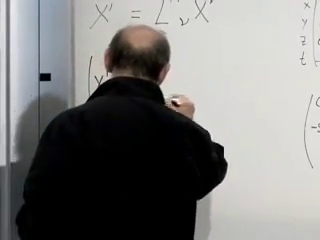
\includegraphics[width=0.8\textwidth]{lecture_06_figure_03.png}\caption{Componentes contravariantes y covariantes, la matriz métrica y el inicio de la contracción invariante.}\lectureframe{00:45:00}\end{figure}

Bajar índices no es un mero adorno. Incorpora los signos necesarios para obtener la norma invariante de Lorentz: \begin{align}
  A_\mu A^\mu
  &=-(A^1)^2-(A^2)^2-(A^3)^2+(A^0)^2,                    \label{eq:l6-norm}\\
  X_\mu X^\mu
  &=t^2-x^2-y^2-z^2.
\end{align} La segunda expresión es el intervalo espacio-temporal invariante desde el origen. Como \(A^\mu\) se transforma igual que \(X^\mu\), su contracción conserva la invariancia.

La notación también enseña una regla útil para llevar la cuenta. Un índice de suma aparece una vez arriba y otra abajo. Por ejemplo: \begin{equation}
  A_\mu A^\mu
  =\eta_{\mu\nu}A^\mu A^\nu.
\end{equation} Los nombres de los índices sumados, o mudos, se pueden cambiar sin alterar la cantidad.

\begin{classroomqa}\audiencequestion{¿Hay que considerar uno de estos vectores como una fila y el otro como una columna? ¿Importa el orden?}\lecturerresponse{Para el cálculo que hacemos, consideremos las cantidades con índices como componentes y dejemos que la métrica efectúe la contracción; no hace falta convertir la discusión en álgebra de operadores con vectores fila y columna. Son números ordinarios, así que el orden no importa. Los operadores que no conmutan requieren más cuidado, pero eso no es lo que tratamos aquí.}\end{classroomqa}

La misma construcción da el producto escalar entre dos cuatro-vectores distintos: \begin{equation}
  A\mathbin{\cdot}B=A_\mu B^\mu=A^\mu B_\mu.
\end{equation} Su invariancia se demuestra sin escribir explícitamente una matriz de Lorentz. Como \(A+B\) y \(A-B\) son cuatro-vectores, los cuadrados de sus normas son invariantes: \begin{align}
  (A+B)^2&=A^2+B^2+2A\mathbin{\cdot}B,\\
  (A-B)^2&=A^2+B^2-2A\mathbin{\cdot}B.
\end{align} Al restarlos se obtiene \begin{equation}
  (A+B)^2-(A-B)^2=4A\mathbin{\cdot}B,                    \label{eq:l6-polarization}
\end{equation}, por lo que \(A\mathbin{\cdot}B\) también es invariante. El factor cuatro se deduce directamente del desarrollo.\editorialnote{Este argumento de la pizarra da la identidad de polarización; escribir explícitamente el factor hace inequívoca la cancelación mencionada oralmente.}

\begin{figure}[H]\centering
\includegraphics[width=0.8\textwidth]{lecture_06_figure_04.png}\caption{Los dos cuadrados invariantes que se usan para aislar el producto escalar de cuatro-vectores distintos.}\lectureframe{00:52:20}\end{figure}

Las cantidades invariantes son ingredientes naturales de las leyes físicas: a diferencia de una componente aislada, conservan el mismo valor de un marco a otro.

\section{Velocidad propia y cuadrimomento}

Consideremos dos sucesos vecinos en la línea de universo de una partícula. Su separación es el cuatro-vector infinitesimal \begin{equation}
  dX^\mu=(dx,dy,dz,dt).
\end{equation} Para una línea de universo temporal, el tiempo propio se define mediante \begin{equation}
  d\tau^2=dX_\mu dX^\mu
  =dt^2-dx^2-dy^2-dz^2.                                  \label{eq:l6-proper-time}
\end{equation} La cuadrivelocidad propia es \begin{equation}
  U^\mu=\frac{dX^\mu}{d\tau}.                            \label{eq:l6-four-velocity}
\end{equation} Mide la tasa de cambio de la posición espacio-temporal con respecto al tiempo propio de la partícula, no con respecto al tiempo coordenado de un marco elegido.

Aunque \(U^\mu\) tiene cuatro componentes, solo tres son independientes. Al dividir la ec.~\eqref{eq:l6-proper-time} por \(d\tau^2\) se obtiene \begin{equation}
  U_\mu U^\mu=1.
\end{equation} Así, la cuadrivelocidad es un vector temporal unitario. La elección dirigida hacia el futuro fija el signo de su componente temporal.

\begin{classroomqa}\audiencequestion{Cuando las velocidades son mucho menores que \(c\), ¿se reduce la cuadrivelocidad a la velocidad ordinaria?}\lecturerresponse{Sus tres componentes espaciales se aproximan a la velocidad ordinaria, mientras que su componente temporal se aproxima a uno en unidades con \(c=1\). La relación se obtiene aplicando la regla de la cadena y calculando \(dt/d\tau\).}\end{classroomqa}

Para cada componente espacial, \begin{equation}
  U^i=\frac{dx^i}{d\tau}
     =\frac{dx^i}{dt}\frac{dt}{d\tau}
     =v^i\frac{dt}{d\tau}.
\end{equation} Dividamos la ec.~\eqref{eq:l6-proper-time} por \(dt^2\): \begin{equation}
  \left(\frac{d\tau}{dt}\right)^2
  =1-v_x^2-v_y^2-v_z^2
  =1-\boldsymbol v^2.
\end{equation} Por tanto, \begin{equation}
  \frac{dt}{d\tau}=\frac{1}{\sqrt{1-\boldsymbol v^2}}
  =\gamma(\lvert\boldsymbol v\rvert),
\end{equation} y \begin{equation}
  U^\mu=(\gamma v_x,\gamma v_y,\gamma v_z,\gamma).
                                                                  \label{eq:l6-u-components}
\end{equation}

\begin{figure}[H]\centering
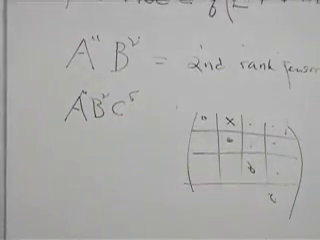
\includegraphics[width=0.8\textwidth]{lecture_06_figure_05.png}\caption{El cálculo con el tiempo propio que da \(dt/d\tau=\gamma\) y relaciona la velocidad propia con la velocidad ordinaria.}\lectureframe{01:02:00}\end{figure}

\begin{classroomqa}\audiencequestion{¿Significa \(dx^2/dt^2\) una segunda derivada, y al elevar al cuadrado un vector se obtienen términos cruzados?}\lecturerresponse{Aquí significa \((dx/dt)^2\), el cuadrado de una primera derivada. Además, \(\boldsymbol v^2\) significa el producto escalar euclídeo \(v_x^2+v_y^2+v_z^2\), no el cuadrado de la suma formal \(v_x+v_y+v_z\); no hay términos cruzados.}\end{classroomqa}

\begin{classroomqa}\audiencequestion{¿Es \(v\) en \(\gamma(v)\) la velocidad relativa de dos marcos de coordenadas o la velocidad de la partícula?}\lecturerresponse{Aquí es la velocidad de la partícula en el marco elegido. La función \(\gamma(v)=1/\sqrt{1-v^2}\) se puede evaluar para cualquier velocidad: en una transformación de Lorentz se evalúa para la velocidad relativa entre marcos; en la cuadrivelocidad, para la velocidad de la partícula.}\end{classroomqa}

Para \(v\ll1\), \(\gamma\simeq1\), así que las componentes espaciales de \(U^\mu\) se aproximan a \(\boldsymbol v\) y \(U^0\) se aproxima a uno. Cuando la velocidad ordinaria se aproxima a la velocidad de la luz, \(\gamma\) y todas las componentes no nulas de la cuadrivelocidad crecen sin límite.

\begin{classroomqa}\audiencequestion{¿No debería \(U^0\) tener unidades de velocidad, en lugar de ser cercano al número uno?}\lecturerresponse{Las unidades desaparecieron al fijar \(c\) igual a uno. Con \(X^0=ct\), se tiene \(U^\mu=(\gamma\boldsymbol v,\gamma c)\), así que la componente temporal se aproxima a \(c\) y \(U_\mu U^\mu=c^2\).}\end{classroomqa}

Para una partícula de masa en reposo \(m\), definamos el cuadrimomento mediante \begin{equation}
  P^\mu=mU^\mu.
\end{equation} En unidades naturales, \begin{equation}
  P^\mu=(\gamma m\boldsymbol v,\gamma m).
\end{equation} A bajas velocidades, las tres primeras componentes se aproximan al momento newtoniano \(m\boldsymbol v\). Al restablecer las unidades se obtiene \begin{equation}
  P^\mu=(\gamma m\boldsymbol v,E/c),
  \qquad E=\gamma mc^2,
\end{equation} y, por tanto, \begin{equation}
  E=mc^2+\frac{1}{2}m\boldsymbol v^2+O(mv^4/c^2).
\end{equation} La componente temporal es la energía en unidades con \(c=1\), o bien la energía dividida por \(c\) si se asignan unidades de momento a las cuatro componentes.

\begin{classroomqa}\audiencequestion{¿Es la velocidad ordinaria \(\boldsymbol v\), con una cuarta componente añadida, un cuatro-vector?}\lecturerresponse{No. La velocidad ordinaria tridimensional no se transforma como un cuatro-vector. El factor \(\gamma\) y la definición mediante el tiempo propio son esenciales; el cuatro-vector es \(U^\mu\), no \(\boldsymbol v\).}\end{classroomqa}

\section{Por qué deben mezclarse los campos eléctrico y magnético}

Ahora nos tomaremos lo que se llamó unas breves vacaciones de la relatividad. Empecemos con la ecuación de movimiento anterior a Einstein y preguntémonos cómo hay que reorganizarla para que sea válida en todos los marcos inerciales. La aceleración ordinaria es la derivada temporal de la velocidad ordinaria. Su análogo tetradimensional es, naturalmente, \begin{equation}
  A^\mu=\frac{dU^\mu}{d\tau}.
\end{equation} A bajas velocidades, sus componentes espaciales se aproximan a la aceleración ordinaria. Dejaremos para más adelante la ecuación relativista completa; primero examinemos la antigua ley de fuerza.

Para una carga \(q\) en campos eléctrico y magnético: \begin{equation}
  \boldsymbol F=m\boldsymbol a
  =q\left(\boldsymbol E+\boldsymbol v\times\boldsymbol B\right).
                                                                  \label{eq:l6-lorentz-force}
\end{equation} El término eléctrico es independiente de la velocidad de la partícula, mientras que el término magnético no lo es.

\begin{figure}[H]\centering
\includegraphics[width=0.8\textwidth]{lecture_06_figure_06.png}\caption{La forma prerrelativista de la ley de fuerza de Lorentz que motiva la combinación de \(\boldsymbol E\) y \(\boldsymbol B\).}\lectureframe{01:18:20}\end{figure}

Supongamos que un observador no ve ningún campo eléctrico, pero sí un campo magnético y una carga en movimiento. La carga siente una fuerza magnética. Sin embargo, en el marco de reposo instantáneo de la carga, \(\boldsymbol v=0\), así que el término magnético de la ec.~\eqref{eq:l6-lorentz-force} se anula. La línea de universo física no se vuelve inercial por el mero hecho de cambiar las coordenadas; por tanto, la fuerza en el nuevo marco debe incluir una contribución eléctrica. Más precisamente, una aceleración de cuatro dimensiones no nula no puede transformarse en cero cambiando de marco inercial, aunque la aceleración tridimensional y sus componentes sí se transformen. \editorialnote{Esta afirmación sobre la aceleración de cuatro dimensiones es la forma invariante del argumento de clase y evita tratar la aceleración ordinaria tridimensional como si fuera invariante de marco.}

Por consiguiente, los campos eléctrico y magnético deben transformarse uno en otro. Juntos tienen seis componentes, así que no forman ni un escalar ni un cuatro-vector. Necesitamos un nuevo objeto que se transforme.

\section{Tensores: una transformación por índice}

Un escalar puede llamarse tensor de rango cero; no tiene índices. Un cuatro-vector es un tensor de rango uno: tiene un índice con cuatro valores posibles. El ejemplo más sencillo de rango dos es un producto: \begin{equation}
  A^\mu B^\nu.
\end{equation} Cada índice tiene cuatro valores, así que el objeto tiene \(4^2=16\) componentes, que se pueden representar como un arreglo \(4\times4\). Un producto de tres vectores, \begin{equation}
  A^\mu B^\nu C^\sigma,
\end{equation}, tiene \(4^3=64\) componentes y es un tensor de rango tres. Los rangos superiores siguen el mismo patrón. El nombre importa menos que la regla que define el objeto.

Si \begin{equation}
  A'^{\mu}=\Lambda^\mu{}_{\nu}A^\nu,
  \qquad
  B'^{\sigma}=\Lambda^\sigma{}_{\tau}B^\tau,
\end{equation}, entonces su producto se transforma como \begin{equation}
  A'^{\mu}B'^{\sigma}
  =\Lambda^\mu{}_{\nu}\Lambda^\sigma{}_{\tau}
   A^\nu B^\tau.
\end{equation}. Esto da la ley que define un tensor contravariante de rango dos: \begin{equation}
  T'^{\mu\sigma}
  =\Lambda^\mu{}_{\nu}\Lambda^\sigma{}_{\tau}T^{\nu\tau}.
                                                                  \label{eq:l6-tensor-transform}
\end{equation} Hay una matriz de Lorentz por cada índice. Los índices repetidos \(\nu\) y \(\tau\) se suman; los índices libres \(\mu\) y \(\sigma\) identifican la componente que se calcula en el marco primado.

\begin{figure}[H]\centering
\includegraphics[width=0.82\textwidth]{lecture_06_figure_07.png}\caption{La transformación de dos vectores y la ley de transformación resultante, con dos matrices, para un tensor de rango dos.}\lectureframe{01:27:15}\end{figure}

Un tensor no tiene por qué ser el producto de un solo par de vectores. Tanto \(A^\mu B^\nu\) como \(A^\nu B^\mu\) obedecen la ley de transformación de los tensores, al igual que su suma y cualquier suma como \begin{equation}
  A^\mu B^\nu+C^\mu D^\nu.
\end{equation} La definición es la ley de transformación, no una factorización particular. Un tensor de rango tres adquiere una tercera matriz de Lorentz, y así sucesivamente.

\section{Tensores simétricos y antisimétricos}

Dos clases de tensores de rango dos serán especialmente útiles. Un tensor simétrico satisface \begin{equation}
  T^{\mu\nu}=T^{\nu\mu},
\end{equation}, de modo que las entradas reflejadas respecto de la diagonal son iguales. Sus cuatro entradas diagonales y las seis entradas a un lado de la diagonal determinan las demás, lo que da \begin{equation}
  4+6=10
\end{equation} componentes independientes.

Un tensor antisimétrico satisface \begin{equation}
  T^{\mu\nu}=-T^{\nu\mu}.                                \label{eq:l6-antisymmetry}
\end{equation}. Al poner \(\mu=\nu\) en la ec.~\eqref{eq:l6-antisymmetry} se obtiene \(T^{\mu\mu}=-T^{\mu\mu}\), así que todas las entradas diagonales se anulan. Las seis entradas de una mitad triangular determinan las otras seis con el signo cambiado. Por tanto, hay exactamente seis componentes independientes.

\begin{figure}[H]\centering
\includegraphics[width=0.82\textwidth]{lecture_06_figure_08.png}\caption{Un arreglo antisimétrico \(4\times4\) completo: ceros en la diagonal y signos opuestos a ambos lados.}\lectureframe{01:34:25}\end{figure}

Ese recuento da la pista. Las tres componentes eléctricas y las tres magnéticas pueden reunirse en un único tensor antisimétrico de rango dos.

\section{El tensor electromagnético}

Ordenemos las etiquetas del espacio-tiempo en filas y columnas como \((1,2,3,0)=(x,y,z,t)\). La matriz escrita en la pizarra es \begin{equation}
  F_{\mu\nu}=
  \begin{pmatrix}
    0    & -B_3 & B_2  & E_1\\
    B_3  & 0    & -B_1 & E_2\\
    -B_2 & B_1  & 0    & E_3\\
    -E_1 & -E_2 & -E_3 & 0
  \end{pmatrix}.                                         \label{eq:l6-field-tensor}
\end{equation} Las posiciones puramente espaciales contienen el campo magnético; las que llevan un índice espacial y uno temporal contienen el campo eléctrico. La antisimetría determina las entradas del triángulo inferior una vez conocidas las del triángulo superior.

\begin{classroomqa}\audiencequestion{¿Son negativas todas las entradas magnéticas, y corresponden las etiquetas a \(x,y,z\)?}\lecturerresponse{Los signos del triángulo espacial superior alternan como se muestra: \(-B_3,+B_2,-B_1\). Las etiquetas \(1,2,3\) corresponden a \(x,y,z\), mientras que \(0\) indica el tiempo. La reflexión respecto de la diagonal invierte todos los signos.}\end{classroomqa}

\begin{figure}[H]\centering
\includegraphics[width=0.82\textwidth]{lecture_06_figure_09.png}\caption{El tensor electromagnético completo con el orden de componentes espaciales primero usado en la lección.}\lectureframe{01:41:05}\end{figure}

La notación convencional es \(F_{\mu\nu}\), en lugar de un \(T_{\mu\nu}\) genérico. El profesor conjetura que la letra podría referirse a Faraday, aunque dice explícitamente que desconoce la historia de esta notación. Aquí lo que importa es la antisimetría y sus seis componentes de campo, no esa conjetura sobre la letra.

\begin{classroomqa}\audiencequestion{¿Representa cada entrada de la matriz la intensidad de un campo en el plano de coordenadas indicado?}\lecturerresponse{Es una componente del tensor electromagnético. Las entradas que incluyen el tiempo son componentes eléctricas, y las entradas espaciales--espaciales codifican componentes magnéticas.}\end{classroomqa}

Dejemos aparte la fila y la columna que llevan el índice temporal. El bloque antisimétrico \(3\times3\) restante es magnético. Sus componentes independientes se pueden recordar cíclicamente: \begin{equation}
  F_{12}=-B_3,
  \qquad F_{23}=-B_1,
  \qquad F_{31}=-B_2.                                   \label{eq:l6-magnetic-cycle}
\end{equation} Partiendo de la primera relación, avancemos cada etiqueta según \(1\to2\to3\to1\). De manera equivalente: \begin{equation}
  F_{ij}=-\epsilon_{ijk}B_k,
\end{equation}, con \(\epsilon_{123}=+1\).\editorialnote{La fórmula de Levi--Civita es la forma estándar y compacta de la regla cíclica desarrollada explícitamente en la pizarra.}

\begin{figure}[H]\centering
\includegraphics[width=0.82\textwidth]{lecture_06_figure_10.png}\caption{Las componentes espaciales cíclicas que codifican el campo magnético en el tensor antisimétrico.}\lectureframe{01:46:20}\end{figure}

Las identificaciones del campo eléctrico son más directas: \begin{equation}
  E_1=F_{10},
  \qquad E_2=F_{20},
  \qquad E_3=F_{30}.
\end{equation}

Por consiguiente, el campo magnético tiene dos identidades útiles. En el espacio tridimensional, se puede asociar un vector axial de tres componentes con un tensor antisimétrico \(3\times3\). Sin embargo, en el espacio-tiempo es solo la parte espacial del tensor de seis componentes \(F_{\mu\nu}\). Esta asociación es propia de tres dimensiones: un tensor antisimétrico \(4\times4\) tiene seis componentes independientes y no se puede identificar con un cuatro-vector.\editorialnote{Bajo rotaciones propias, el campo magnético se comporta como un vector; bajo reflexiones, es más precisamente un vector axial o pseudovector.}

El propósito de esta construcción no es contar componentes por el mero hecho de contarlas. Como \(F_{\mu\nu}\) se transforma como un tensor, una transformación de Lorentz mezcla automáticamente sus componentes eléctricas y magnéticas. En la próxima lección se puede combinar con la cuadrivelocidad y la cuadraceleración para reemplazar la ec.~\eqref{eq:l6-lorentz-force} por una ecuación de movimiento covariante.

\section{Preguntas sobre Einstein y Minkowski}

Los minutos finales pasan del formalismo a la historia de cómo surgió. Las respuestas se ofrecen como recuerdos, no como una historia establecida; esa salvedad forma parte del intercambio.

\begin{classroomqa}\audiencequestion{¿Buscaba Einstein una formulación invariante de Lorentz por razones conceptuales, o lo impulsaron observaciones concretas?}\lecturerresponse{El principio de que las leyes de la naturaleza deben tener la misma forma en todos los marcos inerciales fue central en su razonamiento. También había pruebas experimentales relacionadas con la luz y la imposibilidad de detectar el movimiento a través de un éter, aunque el profesor expresa explícitamente sus dudas sobre qué resultados conocía Einstein o cuánto influyeron en él. La motivación conceptual era que las ecuaciones de Maxwell y la fuerza de Lorentz debían obedecer el principio de relatividad, lo que exige que los campos eléctricos, los campos magnéticos y las componentes de la velocidad se transformen conjuntamente.}\end{classroomqa}

La exposición de Einstein de 1905 no usaba la notación compacta de cuatro-vectores que empleamos aquí. Trabajaba componente por componente y escribía explícitamente los factores necesarios de \(\gamma\) y de la velocidad. Posteriormente, Minkowski organizó geométricamente la misma estructura como un espacio-tiempo tetradimensional.

\begin{classroomqa}\audiencequestion{¿Se resistió Einstein a la formulación del espacio-tiempo de Minkowski, y cuánto tardó Minkowski en proponerla?}\lecturerresponse{El recuerdo que se ofrece en clase es que Einstein no acogió inicialmente con agrado el lenguaje geométrico tetradimensional, pero pronto reconoció su valor. La fecha se da con cautela como aproximadamente dos años después del artículo de 1905, quizá en 1907; el profesor recalca que está recordando la historia, no estableciéndola.}\end{classroomqa}

\begin{classroomqa}\audiencequestion{¿Minkowski era matemático o físico, qué otras contribuciones hizo y recibió influencia de Lorentz o FitzGerald?}\lecturerresponse{No se afirma tener una respuesta segura. No se profundiza en la distinción entre matemático y físico; una corrección del público interrumpe un comentario general sobre otros trabajos de Minkowski, y las posibles influencias se dejan expresamente como inciertas. El punto firme para esta discusión es la decisiva organización de la relatividad que hizo Minkowski mediante la notación geométrica tetradimensional.}\end{classroomqa}

\begin{classroomqa}\audiencequestion{¿Estaban ya presentes en el trabajo de Einstein de 1905 las transformaciones que mezclan \(\boldsymbol E\) y \(\boldsymbol B\)?}\lecturerresponse{Sí, pero escritas componente por componente en vez de como una sola ecuación para el tensor de campo. En clase se las compara con las ecuaciones de Maxwell escritas por componentes: el contenido puede estar presente antes de que una notación compacta revele su estructura común. La contribución de Minkowski fue sistematizar esa estructura en el lenguaje del espacio-tiempo.}\end{classroomqa}

Eso nos devuelve al punto matemático por el que empezamos. Los componentes son indispensables para los cálculos, pero la ley se vuelve inteligible cuando se reconocen como partes de un único objeto que se transforma. La siguiente tarea consiste en usar \(F_{\mu\nu}\) para escribir la ecuación de movimiento de la partícula cargada de una forma que sea la misma en todos los sistemas inerciales.